\section{Architecture}
\label{sec:dspark}
The overview of DSpark is shown in \autoref{fig:model_arch}. Recall from \autoref{eq:latency} that the per-token latency of speculative decoding is $L = (T_{\text{draft}} + T_{\text{verify}})/\tau$.
Autoregressive drafters achieve high $\tau$ but pay $T_{\text{draft}} \propto \gamma$; parallel drafters collapse $T_{\text{draft}}$ to a single pass but sacrifice $\tau$ because each position is predicted independently.
Meanwhile, fixed-length verification wastes $T_{\text{verify}}$ on low-confidence suffix tokens that are almost certain to be rejected.
DSpark addresses these limitations with two complementary components:


\begin{itemize}[leftmargin=*,itemsep=2pt,topsep=4pt]
\item \textbf{Semi-autoregressive generation} (\autoref{sec:semi_ar}). A parallel backbone handles the bulk of draft computation, which keeps $T_{\text{draft}}$ nearly independent of $\gamma$. A lightweight sequential block then injects dependency among draft tokens, improving $\tau$ at minimal additional latency.

\item \textbf{Confidence-scheduled verification} (\autoref{sec:confidence}). A confidence head estimates per-position acceptance probabilities, and a hardware-aware scheduler uses these estimates to prune low-confidence suffix tokens, cutting unnecessary verification compute.
\end{itemize}
% In combination, the two components let DSpark draft better and verify smarter. We detail each below.

\begin{figure}[t!]
    \centering
    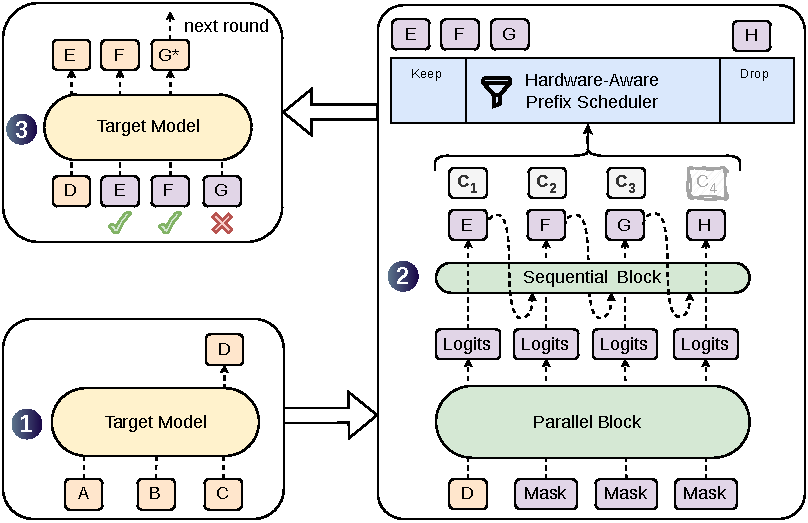
\includegraphics[width=0.9\linewidth]{figs/model_arch.pdf}
    \caption{
        \textbf{The DSpark architecture and decoding cycle.} Given prompt tokens \fbox{ABC}, the target model executes one step to generate the next token \fbox{D}, which serves as the anchor for the drafting phase. Using \fbox{D} as the input, DSpark employs a heavy parallel backbone and a lightweight sequential head to generate draft tokens \fbox{EFGH} along with their corresponding confidence scores \fbox{$c_1$--$c_4$}. The Hardware-Aware Prefix Scheduler then evaluates these scores to retain the prefix \fbox{EFG} and drop the low-confidence token \fbox{H}. 
        Finally, the target model verifies the scheduled prefix in parallel. As illustrated, \fbox{E} and \fbox{F} are accepted while \fbox{G} is rejected, prompting the model to generate a corrected token \fbox{G$^*$} to complete the current round.
    }
    \label{fig:model_arch}
\end{figure}

\subsection{Semi-Autoregressive Generation}
\label{sec:semi_ar}

A parallel drafter produces all $\gamma$ draft logits in one forward pass, so each prediction cannot condition on tokens sampled elsewhere in the block.
When the context admits multiple plausible continuations, e.g., ``of course'' and ``no problem'', a parallel drafter may produce incoherent combinations such as ``of problem'' or ``no course'', because each position marginalizes over all possible predecessors rather than conditioning on the one actually sampled~\citep{gu2018nonautoregressive,pmlr-v162-huang22k}.
Acceptance rate thus decays rapidly along the block, wasting both draft and verification compute.
We therefore adopt a \textbf{semi-autoregressive} structure that splits draft generation into two stages:

\paragraph{Parallel stage.}
A parallel backbone (in our instantiation, DFlash~\citep{chen2026dflash}) runs a single forward pass over the entire block, producing hidden states $h_1, \ldots, h_{\gamma}$ and base logits $U_1, \ldots, U_{\gamma}$.
We make only a minor modification to the original DFlash backbone: instead of feeding an anchor token plus $\gamma$ mask tokens and predicting only the mask positions, we treat the anchor itself as the first prediction position, so $\gamma$ input tokens (anchor $+$ $\gamma{-}1$ masks) yield $\gamma$ draft logits.
This reduces draft computation while maintaining similar draft quality.

\paragraph{Sequential stage.}
The sequential stage supplements the base logits with a prefix-dependent transition bias
$B_k(x_0, x_{<k}, x_k)$, allowing each draft position to condition on previously sampled
tokens within the block. Rather than defining a globally normalized energy model, the
sequential stage induces a causal block distribution through an autoregressive
factorization:
\begin{equation}
P(X \mid x_0)
=
\prod_{k=1}^{\gamma}
p_k(x_k \mid x_0, x_{<k}),
\qquad
p_k(v \mid x_0, x_{<k})
=
\frac{
\exp\!\left(U_k(v) + B_k(x_0, x_{<k}, v)\right)
}{
\sum_{u \in \mathcal{V}}
\exp\!\left(U_k(u) + B_k(x_0, x_{<k}, u)\right)
}.
\label{eq:sequential-factorization}
\end{equation}
Here, $x_0$ denotes the anchor token from the previous verification cycle, $U_k$ is the
base logit vector produced by the parallel backbone at position $k$, and $\mathcal{V}$ is the
vocabulary. At inference time, the sequential block samples left to right according to
$p_k(\cdot \mid x_0, x_{<k})$.
Because this sampling process is inherently sequential, the block must be computationally
lightweight ($T_{\text{sequential}} \ll T_{\text{parallel}}$) so that the overall draft latency
remains dominated by the parallel stage.
We describe two instantiations of the sequential block below.

\begin{itemize}
    \setlength{\itemsep}{10pt}
    \item \textbf{Markov head.} The simplest instantiation restricts $B_k$ to depend only on the immediately preceding token, reducing it to a first-order transition $B(x_{k-1}, x_k)$.
    In principle this is a full $V \times V$ matrix $B$; we approximate it with a low-rank factorization $B = W_1 W_2$, where $W_1 \in \RR^{V \times r}$ and $W_2 \in \RR^{r \times V}$.
    Given the preceding token $x_{k-1}$, the transition bias for position $k$ is:
    \begin{equation}
    B(x_{k-1},\, \cdot\,) = W_1[x_{k-1}] \, W_2 \;\in\; \RR^{V},
    \label{eq:markov}
    \end{equation}
    where $W_1$ serves as an embedding lookup table and $W_2$ as a logit projection.
    The low-rank factorization ($r{=}256$ by default) keeps both storage and per-step compute small, making the sequential loop efficient even for large vocabularies.
    Returning to the earlier example: once position 1 samples ``of'', the Markov head boosts ``course'' and suppresses ``problem'' at position 2, which mitigates the cross-mode collision.

    \item \textbf{RNN head.} The Markov head is memoryless beyond one step—position $k$ cannot access tokens before $x_{k-1}$.
    The RNN head relaxes this by maintaining a recurrent state $s_k$ that accumulates the full prefix history within a block.
    At each step, the module concatenates the current state $s_{k-1} \in \RR^{r}$, the previous token embedding $W_1[x_{k-1}] \in \RR^{r}$, and the backbone hidden $h_k \in \RR^{d}$ into an input vector $z_k = [s_{k-1};\, W_1[x_{k-1}];\, h_k] \in \RR^{2r+d}$, then applies a single gated update:
    \begin{equation}
    \begin{aligned}
    s_k = \sigma(W_g\, z_k)& \odot s_{k-1} \;+\; \bigl(1 - \sigma(W_g\, z_k)\bigr) \odot \tanh(W_c\, z_k), \label{eq:rnn}\\
    &B_k(x_{<k},\, \cdot\,) = W_2^\top\, \tanh(W_o\, z_k),
    \end{aligned}
    \end{equation}
    where $W_g, W_c, W_o \in \RR^{r\times(2r+d)}$ are jointly parameterized by a single linear projection that is split into gate, candidate, and output components.
    The state $s_0$ is initialized to zero.
\end{itemize}

\subsection{Confidence-Scheduled Verification}  
\label{sec:confidence}  

The semi-autoregressive architecture enables DSpark to generate large draft blocks efficiently. However, producing more draft tokens does not automatically translate to higher end-to-end speedups. Indiscriminately verifying the full draft block can actually degrade overall system throughput, especially in high-concurrency scenarios~\citep{liu2024turbospec,hu2026echo}.

This performance bottleneck stems from two interacting factors. 
First, on the data side, draft acceptance rates inherently vary across domains: structured text like code naturally yields high acceptance, whereas open-ended chat has significantly lower acceptance~\citep{xia-etal-2024-unlocking,abramovich2026speed}.
Second, on the system side, the actual cost of verifying an extra token depends strictly on the engine load. Under light system load, an extra verification incurs minimal penalty even if rejected. However, under high-concurrency deployments, every unnecessary verification occupies target model batch capacity that could otherwise serve other active requests~\citep{liu2024optimizing, wu-etal-2025-tetris}.

Therefore, fully unlocking the potential of large draft blocks requires a unified mechanism that routes target model compute only toward tokens with a positive expected return. DSpark achieves this by coupling a \textbf{confidence head} (\autoref{sec:conf_head}) that predicts prefix survival probabilities, with a \textbf{hardware-aware prefix scheduler} (\autoref{sec:scheduler}) that dynamically determines the optimal verification lengths based on current system load.

\subsubsection{Confidence Head}
\label{sec:conf_head}
Drawing inspiration from~\citet{huang2024specdec++,wang2025end}, the confidence head outputs a scalar   $c_k \in (0, 1)$ for each draft position $k$. Crucially, $c_k$ models the \textit{conditional} probability that the draft token at position $k$ will survive target verification, given that all preceding tokens in the block have been accepted.  
The architecture features a lightweight linear projection followed by a sigmoid function:  
\begin{equation}  
c_k = \sigma\bigl(w^\top [h_k;\, W_1[x_{k-1}]]\bigr),  
\label{eq:confidence}  
\end{equation}  
where $h_k$ is the hidden state of the backbone and $W_1[x_{k-1}]$ is the Markov Embedding from the previous draft token. We supervise $c_k$ using the analytical acceptance rate per-step $c_k^*$. This rate is determined by the total variation distance between the draft distribution $p_k^d$ and the target distribution $p_k^t$:  
\begin{equation}  
c_k^* = 1 - \tfrac{1}{2}\|p_k^d - p_k^t\|_1.  
\label{eq:accept_rate}  
\end{equation}

  
\paragraph{Post-hoc Calibration.}  
Unlike threshold-based verification heuristics~\citep{huang2024specdec++,li-etal-2024-eagle,zhang2026pacer}, which only require confidence scores to correctly rank draft token qualities, our hardware-aware scheduling approach (detailed in \autoref{sec:scheduler}) precisely requires the absolute magnitudes of the cumulative acceptance probabilities to compute the expected acceptance length $\tau$. Because neural confidence estimates are often overconfident~\citep{guo2017calibration,ovadia2019can}, using the raw confidence scores directly would distort the throughput estimation, leading to suboptimal scheduling.  
  
To address this, we introduce \textbf{Sequential Temperature Scaling (STS)}. Because each $c_i$ models a conditional probability, the chain rule dictates that the joint probability of a draft prefix being accepted factorizes into the cumulative product $\prod_{i \leq k} c_i$. Using a held-out validation set, STS calibrates this joint probability consecutively from left to right. Specifically, at each position $k \in \{1,\dots,\gamma\}$, we perform a simple 1D grid search to find the optimal temperature scalar that minimizes the Expected Calibration Error (ECE)~\citep{naeini2015obtaining} of the cumulative product, keeping the already-calibrated scores of all preceding positions fixed. Crucially, temperature scaling is an order-preserving transformation: it rectifies the predicted probabilities to match empirical acceptance rates without disrupting the relative draft token rankings learned by the confidence head.

\subsubsection{Hardware-Aware Prefix Scheduler}  
\label{sec:scheduler}

\begin{algorithm}[t]
\caption{Hardware-Aware Prefix Scheduler}    
\label{alg:prefix-scheduler}    
\begin{algorithmic}[1]    
\REQUIRE Active requests $r \in \{1,\dots,R\}$; confidence sequence $c_{r,1},\dots,c_{r,\gamma}$ per request; profiled step curve $\text{SPS}(B)$    
\ENSURE Selected per-request prefix lengths $\ell^*_1,\dots,\ell^*_R$    
\FOR{$r = 1$ \TO $R$}    
  \STATE Compute prefix survival probabilities: $a_{r,j} \gets \prod_{i \leq j} c_{r,i}$ for $j = 1,\dots,\gamma$    
\ENDFOR    
\STATE Construct candidate space $\mathcal{E} \gets \{(r, j) \mid a_{r,j} > 0\}$ and sort descending by $a_{r,j}$    
\STATE Initialize states: $\ell_r \gets 0$ for all $r$; Batch size $B \gets R$; Expected accepts $\tau^* \gets R$    
\STATE Initialize tracking: $\Theta_{\text{best}} \gets R \cdot \text{SPS}(R)$; Selected lengths $\ell^*_r \gets 0$ for all $r$    
\FOR{each $(r, j) \in \mathcal{E}$ in sorted order}    
  \STATE $\ell_r \gets j$; $B \gets B + 1$; $\tau^* \gets \tau^* + a_{r,j}$    
  \STATE Current throughput $\Theta \gets \tau^* \cdot \text{SPS}(B)$    
  \IF{$\Theta > \Theta_{\text{best}}$}    
    \STATE $\Theta_{\text{best}} \gets \Theta$; Update selected lengths $\ell^*_r \gets \ell_r$
  \ELSE
    \STATE \textbf{break}
  \ENDIF    
\ENDFOR    
\RETURN $(\ell^*_1,\dots,\ell^*_R)$ achieving $\Theta_{\text{best}}$    
\end{algorithmic}    
\end{algorithm}

Prior methods~\citep{huang2024specdec++,li-etal-2024-eagle} typically apply a static threshold to confidence scores to determine verification length. While effective under isolated, single-request assumptions, static thresholds can be suboptimal in high-concurrency production systems, where the utility of verifying a draft token depends heavily on the current system load.  
  
To address this, we formulate verification length selection as a global throughput maximization problem~(\autoref{alg:prefix-scheduler}). Consider a batch of $R$ active requests. For request $r$, let $c_{r,1},\dots,c_{r,\gamma}$ be the per-position confidence estimates, and let $\ell_r \in \{0,\dots,\gamma\}$ denote the scheduled verification length. Because speculative decoding dynamically accepts draft tokens only as a continuous prefix, the survival probability of a token at position $j$ is the cumulative product $a_{r,j} = \prod_{i \leq j} c_{r,i}$.  
  
In a single verification step, the total batch size (measured in tokens) sent to the target model is $B = \sum_{r=1}^{R} (1 + \ell_r)$, and the expected number of successfully accepted tokens is $\tau = \sum_{r=1}^{R} \bigl(1 + \sum_{j=1}^{\ell_r} a_{r,j}\bigr)$. 
% In most real online serving scenarios, the average context length is far below 1M tokens, so the context length has only a minor impact on decode performance for DeepSeek-V4. Moreover, in prefill-decode disaggregated deployment, the decode load balancer keeps both the number of requests and the total context length roughly balanced across different data-parallel (DP) ranks. We therefore assume that the engine throughput depends only on $B$. 
Under a simplifying assumption\footnote{In practical serving scenarios, average context lengths remain well below extremes (e.g., 1M tokens), making their impact on decode latency marginal for highly optimized architectures like DeepSeek-V4. Moreover, in prefill-decode disaggregated deployments, decode load balancers keep both request counts and total context lengths roughly balanced across data-parallel (DP) ranks. This effectively amortizes sequence-length variance, allowing us to safely assume that engine throughput depends predominantly on the verification batch size $B$.}, let $\text{SPS}(B)$ denote the engine throughput, measured in steps per second, for a given forward-pass batch size $B$. Crucially, this capacity curve is profiled once during engine initialization and stored as a lightweight cost table. Our scheduler then aims to maximize the expected system-wide token throughput $\Theta = \tau \cdot \text{SPS}(B)$ by dynamically selecting verification lengths $\ell_1,\dots,\ell_R$.
  
Although finding the global maximum of $\Theta$ appears to be a combinatorial search, the objective structure allows for an efficient greedy solution. Because $a_{r,j}$ is monotonically non-increasing with respect to $j$ (i.e., $a_{r, j} \le a_{r, j-1}$), the marginal gain in expected accepted tokens for extending request $r$'s verification length from $j-1$ to $j$ is exactly $a_{r,j}$. This monotonicity ensures that sorting candidate tokens globally by $a_{r,j}$ naturally respects intra-block prefix dependencies. Consequently, if the total verification batch size $B$ were fixed, the optimal allocation $\{\ell_r\}$ would be determined by greedily selecting the draft tokens with the highest survival probabilities from the global pool of all $\{a_{r,j}\}$.

Building on this insight, the optimization can be evaluated along this greedy admission path. We first globally sort all valid prefix extensions in descending order of survival probability. To dynamically determine the optimal target batch size $B$, we incrementally admit tokens from this sorted pool, updating the expected throughput $\Theta$ via an lookup from the cost table. 

Lossless speculative decoding strictly requires the \textit{non-anticipating property}: admission decisions must not depend on future candidate tokens~\citep{pmlr-v202-leviathan23a,chen2023accelerating}. Because our confidence head relies on the Markov feature of the previously sampled token, computing the next survival probability $a_{r,k+1}$ explicitly requires the instantiated candidate $x_{r,k}$. A retrospective global search would thus inadvertently leak $x_{r,k}$ into the admission decision for step $k$, introducing selection bias~(we provide a concrete counterexample demonstrating this theoretical violation in \autoref{app:counterexample}).

To enforce strict causality, the scheduler (\autoref{alg:prefix-scheduler}) employs an early-stopping mechanism. By breaking the greedy search immediately when the throughput drops ($\Theta \le \Theta_{\text{best}}$), the truncation decision relies solely on the prefix processed up to that exact step. This isolates the admission event from future tokens, ensuring exact target-distribution recovery. Note that this stepwise early-stopping yields the global maximum throughput if and only if the objective $\Theta$ is unimodal, which implicitly assumes a smoothly decaying hardware capacity curve. We address the engineering adaptations required for real-world, non-smooth $\text{SPS}$ characteristics and asynchronous system pipelines in \autoref{sec:scheduler_in_practice}.

\subsection{Training}
\label{sec:training}

During training, we randomly sample multiple anchor positions from each target sequence to form $\gamma$-token blocks as training data.
The target model is frozen throughout training; the draft model shares its embedding layer and language modeling head and keeps them frozen, updating only the backbone drafter, sequential block, and confidence head.

The training objective consists of three terms: a cross-entropy loss $\Ll_{\text{ce}}$, a distribution-matching loss $\Ll_{\text{tv}}$, and a confidence loss $\Ll_{\text{conf}}$.
All three are position-weighted by $w_k = \exp(-(k{-}1)/\gamma)$~\citep{chen2026dflash}, which emphasizes earlier block positions that contribute more to the expected acceptance length under prefix-based verification.
The cross-entropy loss $\Ll_{\text{ce}}$ trains the drafter to predict the correct next token:
\begin{equation}
\Ll_{\text{ce}} = -\sum_{k=1}^{\gamma} w_k \log p^d_{k}(x_k^*),
\end{equation}
where $x_k^*$ is the ground-truth token and $p^d_k$ is the draft distribution.
The distribution-matching loss $\Ll_{\text{tv}}$ penalizes the total variation distance between the draft and target distributions:
\begin{equation}
\Ll_{\text{tv}} = \sum_{k=1}^{\gamma} w_k \|p_k^d - p_k^t\|_1.
\end{equation}
Since the total variation distance is a direct proxy for the acceptance rate: the per-step acceptance probability equals $1 - \frac{1}{2}\|p^d - p^t\|_1$~\citep{pmlr-v202-leviathan23a}, minimizing $\Ll_{\text{tv}}$ directly maximizes the expected acceptance rate.

The confidence loss $\Ll_{\text{conf}}$ is a binary cross-entropy that trains the confidence head to predict the soft acceptance label $c_k^*$ from \autoref{eq:accept_rate}:
\begin{equation}
\Ll_{\text{conf}} = -\sum_{k=1}^{\gamma} w_k \bigl[c_k^* \log c_k + (1 - c_k^*) \log(1 - c_k)\bigr].
\end{equation}
The overall objective is a weighted combination of the three terms~(with default weights $\alpha_{\text{ce}} = 0.1$, $\alpha_{\text{tv}} = 0.9$, $\alpha_{\text{conf}} = 1.0$):
\begin{equation}
\Ll = \alpha_{\text{ce}}\,\Ll_{\text{ce}} + \alpha_{\text{tv}}\,\Ll_{\text{tv}} + \alpha_{\text{conf}}\,\Ll_{\text{conf}}
\label{eq:loss}
\end{equation}


